%\documentclass[reprint,amsmath,amssymb,superscriptaddress,prl,showpacs,onecolumn]{revtex4-1}
\documentclass[reprint,amsmath,amssymb,superscriptaddress,showpacs,pre]{revtex4-1}
\usepackage{graphicx}% Include figure files
\usepackage{dcolumn}% Align table columns on decimal point
\usepackage{bm}% bold math
\usepackage{color}
\usepackage{epstopdf} 
\usepackage{subfig}
\usepackage{amsmath,amsfonts,amssymb}
\usepackage{amsthm}
\usepackage{hyperref}
\usepackage{algorithm}
\usepackage{algorithmic}
%\usepackage{physics}
\usepackage{lineno}
\linenumbers

%\usepackage{pstricks}
\usepackage{braket}
\DeclareMathOperator\atanh{arctanh}


%\usepackage[hypertex]{hyperref}
\usepackage[sans]{dsfont}

\usepackage{epstopdf}
\usepackage{ulem}
\usepackage{hyperref}
\usepackage{mathbbol}
\usepackage{bbm}


\let\originalleft\left
\let\originalright\right
\renewcommand{\left}{\mathopen{}\mathclose\bgroup\originalleft}
\renewcommand{\right}{\aftergroup\egroup\originalright}
%\newcommand{\bra}[1]{\ensuremath{\left< #1\right|}}
%\newcommand{\ket}[1]{\ensuremath{\left|#1\right>}}
\newcommand{\ovl}[2]{\ensuremath{\left\langle #1\middle|#2\right\rangle}}
\newcommand{\ie}{\emph{i.e.}}
\newcommand{\eg}{\emph{e.g.}}
\newcommand{\cf}{cf.}
\newcommand{\cp}{\emph{cp.}}
%\newcommand{\braket}[2]{\left< #1,#2\right>}
%%\newcommand{\<}{\langle}
%%\renewcommand{\>}{\rangle}
\providecommand{\abs}[1]{\left|#1\right|}
\providecommand{\norm}[1]{||#1||}
\newcommand{\arctanh}[1]{\mathrm{arctanh}#1}
\newcommand{\Sign}[1]{\mathrm{Sign}#1}

\def\<{\langle}
\def\>{\rangle}
\def\vx{\vec x}
\def\vh{\vec h}

\newcommand{\ud}{\mathrm{d}}
\newcommand{\etal}{\textit{ et. al. }}
\newcommand{\Ham}{\mathcal{H}}
\newcommand{\B}{\beta}
\def\matF{{\mathbb F}}
\def\Jij{J_{ij}}

\def\Imat{\mathbb{I}}
\def\ext{\qopname\relax m{ext}}

\newcommand{\mi}{\mathrm{i}}
\DeclareMathOperator{\Tr}{Tr}

%%%% 

\newcommand{\ddroit}{\textrm{d}}
% \newcommand{\eexp}{\text{e}}
%\newcommand{\ie}{\emph{i.e.}$\;$}
%\newcommand{\eg}{\emph{e.g.}$\;$}
\newcommand{\Ptot}{P(A_1\ldots A_L)}
\newcommand{\xz}{\vec{x}_0}
\newcommand{\xo}{\vec{x}_1}
\newcommand{\xt}{\vec{x}_2}
\newcommand{\Lam}{\bm{\Lambda}}
\newcommand{\Sig}{\bm{\Sigma}}
\newcommand{\Sigmone}{\bm{\Sigma^{-1}}}
\def\fonetwo{\frac 1 2}
\def\Cmone{C^{-1}}
\def\Lambtwo{\Lambda^2} 
\def\tildex{\tilde{x}}
\newcommand{\HRule}{\rule{\linewidth}{0.5mm}}
\newcommand{\Xk}[1]{X^{\{#1\}}}
\newcommand{\xk}[1]{\vec{x}_{#1}}


\begin{document}
\title{Inference of global coevolutionary models from hierarchical correlated data. }

\author{Edwin Rodriguez Horta} 
%\email{erodriguezh1990@gmail.com}
\affiliation{Group of Complex Systems and Statistical Physics, Department of Theoretical Physics, University of Havana, Cuba}
\affiliation{Laboratoire de Biologie Computationnelle et Quantitative (LCQB), Institut de Biologie Paris-Seine}
\author{Pierre Barrat-Charlaix} 
%\email{ p.barrat@live.fr }
\affiliation{Biozentrum, University of Basel, 4056 Basel, Switzerland}
\author{Martin Weigt} 
\affiliation{Laboratoire de Biologie Computationnelle et Quantitative (LCQB), Institut de Biologie Paris-Seine}
%\email{martin.weigt@upmc.fr}
\author{Alejandro Lage} 
%\email{ale.lage@gmail.com}
\affiliation{Group of Complex Systems and Statistical Physics, Department of Theoretical Physics, University of Havana, Cuba}
\date{\today}
%\pacs{05.60.Gg, 03.65.Xp, 72.10.-d, 87.15.hj}

%Quantum transport (general physics)
%Tunneling (general physics)
%Theory of electronic transport (cond mat)
%Transport dynamics (biomolecules)

\begin{abstract}
The Inverse problem of Statistical Physics infers maximum-entropy  models  compatibles with a corresponding set of empirical averages extracted from a high-dimensional dataset of equilibrium configurations. Practical interest extended these methods to non-equilibrium data  like  time series, where detailed balance does not hold. However, in several applications, data samples  result from evolutionary processes and the relation between configurations is conditioned by a hierarchical structure of the population. This makes sample statistics a superposition of  signals coming from both: internal configuration correlations and relatedness correlations produced by common evolutionary  history, typically represented by a tree. How to disentangle both sources of correlation for a better parameter inference is an open question to explore. Here we propose an approach  where the  evolutive process through a phylogenetic tree is described by  a  multivariate Ornstein-Uhlenbeck dynamics characterized by  gaussian propagator and stationary distributions. Inference of these distributions from  phylogenetic non-independent samples is solved in a Bayesian framework. This procedure can be  extended to discrete variables by using a binary representation of data and approximating  binary sates by continuous variables. Our method proposes a possible way for  a better estimation of both, equilibrium and dynamic parameters, making  applications more accurate.


  
\end{abstract}

\maketitle


\section{\label{sec:int} Introduction}
%\label{sec:int}
Theory and applications of the inverse problem of statistical physics has had great development in recent years since the availability of large amounts of data on a microscopic scale produced by the continuous technological progress. In this context statistical physics paths: from model parameters to  observables, is reversed, toward find global models which describe the statistics of  a set of observed  configurations \cite{Inverse_problem_Berg}. 

Most of the work has been focus in equilibrium reconstruction , where the aim is to learn max Entropy models, Boltzman distribution, from independent and identically distributed equilibrium configurations. Another kind of methods deal with parameters learning from either time series data or from samples of the non-equilibrium steady state: non-equilibrium reconstruction.

Less effort has been done for data biased by population structured signal, where  samples  are not independent because of presence of relatedness between configurations. These structure could be for instance of  geographical or demogrhapic  nature in a population or  phylogenetic  nature  related to a evolutionary processes shaping trait variation among species.  Here we are going to deal with data given by sequences phylogenetically related  through a tree, which describes the hierarchical correlation between configurations. An important problem is the  distinction   of patterns induced by species traits or by phylogeny. 

Our source of inspiration came from the inverse problem in proteins \cite{Inverse_problem_proteins}, where  covariance signal present in an alignment of homologous proteins is described via Potts model. This covariance signal is assumed a consequence of phenotypics constraints like protein structure and function. However it is known that phylogeny relationships in homologous sequences  contaminate the statistics of  the alignment used to learn the equilibrium model. Therefore a direct inference on this alignments  leads to the existence of Potts parameters that attempt to model the full biased statistics limiting their capacity to predict phenotypic properties.

 To define and solve the inverse problem of statistical physics for data samples with hierarchical  relatedness structure is the aim of this work. 

Main difficulties to address  this kind of problem  come from the necessity to use  a proper global evolutionary model which describes the relation between sequences edge connected in a tree and the discrete  characters of data variables which makes certain calculations intractable \cite{entropy_paper}. 

Here we  adopt an approximation where we forget about the discrete nature of variables and model them by continuous variables instead. This transforms the Potts model into a Gaussian distribution \cite{Baldassi}, making the design of a global propagator tractable. We propose a model of evolution described by a multivariate Ornstein-Uhlenbeck process \cite{gardiner}, which is used  to generate evolutionary related data given an arbitrary phylogenetic tree. The corresponding inverse problem became in the inference of the Gaussian potential (Potts parameters) from the knowledge of tree leaves configurations and the dynamics of evolution. 

To this aim, we first review in section \ref{sec:ornstein_uhlenbeck_dynamics}, main characteristics of a multivariate Ornstein-Uhlenbeck process. In section \ref{evolutionary process} we describe the evolutionary process, describing the algorithm used to generate data phylogenetically biased. The statement of the problem in a Bayesian framework is shown in section \ref{statement of the problem}. Section \ref{methods} is dedicated to describe methodology used to solve the inverse problem. Results for evolution of continuos variable sequences and  the application for configuration of discrete variables is presented in section \ref{Results}. Finally the conclusion and outlook in \ref{conc}.

\section{\label{sec:ornstein_uhlenbeck_dynamics}Short summary about Multivariate Ornstein-Uhlenbeck process}
%\label{sec:ornstein_uhlenbeck_dynamics}
Let consider a system characterized by a vector $\mathbf{x}$ with an equilibrium probability distribution given by
\begin{equation}
P(\mathbf{x}) =\frac 1 Z \exp \left\lbrace -\Ham(\mathbf{x}) \right\rbrace \;\; \mbox{with } \Ham(\mathbf{x}) =\frac{1}{2} \left\lbrace \mathbf{x}^T \bm J \mathbf{x}+ \mathbf{h} \cdot \mathbf{x} \right\rbrace \label{eq:equil}
\end{equation}
where the degrees of freedom $x_i \in \mathbb R, i\in [1\ldots N]$ are continuous variables, and the interactions among them $\Jij$ are fixed, but randomly selected 
from a given ensemble of symmetric positive definite matrices. The vector $\mathbf{h}$ describes a local field which shift a  equilibrium configuration of a zero centered   harmonic potential ($ \mathbf{x}^T \bm J \mathbf{x}$) , for simplicity we going to assume $\mathbf{h}=\mathbf{0}$ .

The Langevin equation for  non-massive $N$-dimensional particles with position $\mathbf{x} = (x_i),\;\;i\in\{1\ldots N\}$   interacting according to the Hamiltonian \ref{eq:equil} take the form:

\begin{equation}
\gamma \frac{\ddroit \mathbf{x} }{\ddroit t} = - \bm J \mathbf{x}  + \mathbf{\xi}(t)
\end{equation}
which represent  a multivariate Ornstein-Uhlenbeck   process, being $ \mathbf{\xi}(t)$ an stochastic term and $\gamma$ the viscosity.

Modeling the stochastic term $\xi_i(t)$ as a zero mean Gaussian white noise with variance $\langle \xi_i(t)\xi_j(t') \rangle = 2 K_B T\gamma\delta(t-t')$ that satisfies the fluctuation-dissipation relation, we obtain  the Ito stochastic differential equation for a multivariate O-U process \cite{singh2017multiOU}:
\begin{equation}
\ddroit x_i = -J_{ij}'x_j dt + \left( \sqrt{2 D}\right) _{ij} dW_j
\end{equation}

where:
\begin{itemize}
	\item $dW_j=\xi_j(t) dt$ represent a stochastic Wiener process. 
	\item $J_{ij}'=\frac{J_{ij}}{\gamma}$ is a stiffness stable matrix of mean regression rates.
	\item $D_{ij}=\frac{KT}{\gamma}\delta_{ij}$ is a symmetric positive definite matrix of diffusions coefficients.  
\end{itemize}

It can be shown that the corresponding Fokker-Planck equation is


\begin{equation}
\partial_t P_{1|1}=\hat{L} P_{1|1} 
\end{equation}
where  $P_{1|1}\equiv P( \mathbf{x}', t'|\mathbf{x}, t)$ is the probability density of displacement from $ \mathbf{x}$ at time $t$ to $ \mathbf{x} '$ at time $t'$, and $\hat{L} $ is the  Fokker-Planck operator given by:

\begin{equation}
\hat{L}( \mathbf{x})=-\frac{\partial}{\partial x_i}J_{ij}' x_j+\frac{\partial^2}{\partial x_i\partial x_j}D_{ij}
\end{equation}
The stationary solution for the Fokker-Planck equation $\hat{L} P_{eq}( \mathbf{x})=0$ is:
\begin{equation}
P_{eq}( \mathbf{x}) = \frac{1}{\sqrt{(2\pi)^N \vert \bm{C}\vert}}\exp\left\{ -\frac{1}{2} \mathbf{x}^T\bm{C}^{-1} \mathbf{x} \right\}
\end{equation}
which is a zero mean Gaussian distribution with $\bm C=\left\langle  \mathbf{x}  \mathbf{x}^T\right\rangle $ as the covariance matrix. If from the beginning we set $\mathbf{h}\neq\mathbf{0}$ we get a Gaussian distribution with mean value shift from zero and covariance matrix $\bm C=\left\langle \mathbf{x} \mathbf{x}^T\right\rangle- \left\langle \mathbf{x} \right\rangle \left\langle \mathbf{x} \right\rangle$.


The solution for the  Fokker-Planck equation is 
\begin{eqnarray}
\nonumber
\lefteqn{P(\mathbf{x} ' | \mathbf{x} , \Delta t) =\frac{1}{\sqrt{(2\pi)^N(1-e^{-2\Delta t})\vert\bm{\Sigma}^{-1}\vert}}}\\%\nonumber
&&\times \exp\left\{ -\frac{1}{2}(\mathbf{x} '-\bm{\mu})^T\bm{\Sigma}^{-1}(\mathbf{x} '- \bm{\mu}) \right\}
\label{eqn:multiOU}
\end{eqnarray}

where 
$$ \bm{\mu} = \Lam \mathbf{x}, \qquad \bm{\Sigma} = \bm{C} - \Lam\bm{C}\Lam, \qquad \Lam = e^{-\bm{\frac{J}{\gamma}}\Delta t}, \Delta t=t-t'$$ 
Matrices $\bm J'$, $\bm C$ and $\bm D$ are not independent but are related by the Liapunov stationary condition :
$$\bm J' \bm C+(\bm C \bm J')^T=2 \bm D$$
Using the Liapunov condition and setting $kT=1$ we get 

\begin{equation}
\bm J=\bm C^{-1}
\end{equation}

Particles evolves under potential  $V(x)=\frac{1}{2}\mathbf{x}^T\bm{C}^{-1}\mathbf{x} = \frac{1}{2}\sum_{i,j} J_{ij}x_i x_j$ and the evolutionary process leads to stationary distribution similar to \ref{eq:equil} .

Another important feature  of the Ornstein-Uhlenbeck process based in it's Gauss-Markov property ensures that the times correlation function obeys the linear regression theorem

\begin{equation}
\bm G(t-t')\equiv \left\langle \mathbf{x}(t)\mathbf{x}(t')\right\rangle= e^{-\frac{\bm{ J}}{\gamma}\Delta t} \bm C=\Lam \bm{C}
\end{equation}

describing the covariance of configurations $\mathbf{x}$ and $\mathbf{x}'$ separated in time by $\Delta t$.



\section{Evolutionary process}
\label{evolutionary process}
To simulate an evolutive process for a  multivariate Ornstein-Uhlenbeck dynamics, we must use the propagator \ref{eqn:multiOU} wich provide the probability of observing sequence $\mathbf{x}'$ knowing that it has sequence $\mathbf{x}$ as an ancestor at a time $\Delta t$ in the past. 

An equivalent  method   to generate  a discrete sampling of a path made by  a sequence of states at times $t_n= n \Delta t$ can be obtained from the iteration:
\begin{equation}
\mathbf{x}_{n+1}=\Lam \mathbf{x}_n+\sqrt{\Sigma}\xi_n
\label{eq:evol}
\end{equation}
where $\xi_n\sim N(0,1)$ is an $N-dimensional$ uncorrelated normal variate with zero mean and unit variance.

In this context  $\gamma$ parameter  is the inverse of mutation rate, $\Delta t/\gamma$ is the number of proposed mutations in the interval $\Delta t$ and  potential $\bm J$ determine  how probable is the mutation (if we assume variation in the potential as fitness score).

\subsection{Phylogenetic correlated samples}
Given an  ancestor  configuration $\mathbf{x}_0$,  extracted randomly from the equilibrium distribution (\ref{eq:equil}),  phylogenetic correlated sequences can be generetaded   following the algorithm \ref{alg_1} ,  for simplicity we adopted a binary and homogeneous tree where all branches have the same length.

\begin{algorithm} [H]
			\caption{Generates tree of evolved vectors $T = \{\vx_0, \vx_{1,1}, \vx_{1,2}, \ldots\}$}
				\label{alg_1}
	\begin{algorithmic}[1]
		\REQUIRE Root $\mathbf{x}_0$, branching events $K$, distance to mutants $\Delta t$.
		\ENSURE Returns $T$
		\STATE $T = \{ \mathbf{x}_0 \}$  
		\STATE $L = \{\mathbf{x}_0 \} $  \COMMENT{Leaves of the tree (the last added nodes)}
		\FOR{$(k=1; k<K+1; k+=1;)$}
		\STATE $L_{new} = \{\}$ 
		\FOR{($\mathbf{x}$ in $L$)} 
		\STATE $\mathbf{x}_{\mbox{child1}} = \mbox{Ornstein-Uhlenbeck-evolve}(\mathbf{x}, \Delta t)$
		\STATE $\mathbf{x}_{\mbox{child2}} = \mbox{Ornstein-Uhlenbeck-evolve}(\mathbf{x}, \Delta t)$
		\STATE Append $T \leftarrow= \{\mathbf{x}_{\mbox{child1}}, \mathbf{x}_{\mbox{child2}}\}$
		\STATE Append $L_{new} \leftarrow= \{\mathbf{x}_{\mbox{child1}}, \mathbf{x}_{\mbox{child2}}\}$
		\ENDFOR
		\STATE $L = L_{new}$
		\ENDFOR
		\RETURN $T = \{\mathbf{x}_0, \mathbf{x}_{1,1}, \mathbf{x}_{1,2}, \ldots\}$
	\end{algorithmic} 
\end{algorithm}

The step named Ornstein-Uhlenbeck-evolve$(\mathbf{x},\Delta t)$, carries out a Ornstein-Uhlenbeck evolution (\ref{eq:evol}) starting at configuration $\mathbf{x}$  for a time $\Delta t$. 

The phylogenetic bias present at leaves of the tree depend of the time interval $\Delta t$, the mutation rate $1/\gamma$ and the potential $\bm J$.  Two configurations linked by  OU dynamics (\ref{eq:evol})   are independent  if $\bm J\Delta t /\gamma\rightarrow \infty$ being $\Lambda\rightarrow 0$. Let define the  characteristic time $\Delta t_c$ as the amount of time necessary for an exponential decay of the  quantity   $\Lambda$ by the factor $\frac{1}{e}$, to this  $\bm J\Delta t_c/\gamma \rightarrow 1$.  As $\bm J$ is a matrix  the previous condition became  in $\lambda_{max}\Delta t_c /\gamma\rightarrow1$, where  $\lambda_{max}$  is the  maximum eigenvalue of $\bm J$, describing it's higher grow direction.  We going to  arbitrary define that two configuration remain correlated  if the sampling interval between them satisfy $\Delta t \ll\Delta t_c$. 

Similarly we assume  that contemporary sequences in a tree are   under a strong phylogenetic correlated regime, when the  path time between most distant sequences is lower than characteristic time $\Delta t_c$ . For a binary homogeneous tree with  $K$ branching events this condition became $\Delta t \ll \frac{\Delta t_c}{2*K}$.

 Alternatively if we consider $\bm J$ and $\Delta t$  fixed the same criteria allows us to define the  parameter $\gamma_c\rightarrow \lambda_{max}\Delta t $  as the threshold value for $\gamma$  above which two sequences are considered correlated. For a binary homoneous tree $\gamma_c\rightarrow \lambda_{max}2*K\Delta t $ determine the  characteristic value for the inverse of mutation rate. Tunning the mutation rate respect $1/\gamma_c$ we going to generate sequences with distinct levels of phylogenetic bias. 


\begin{figure}[!htb]
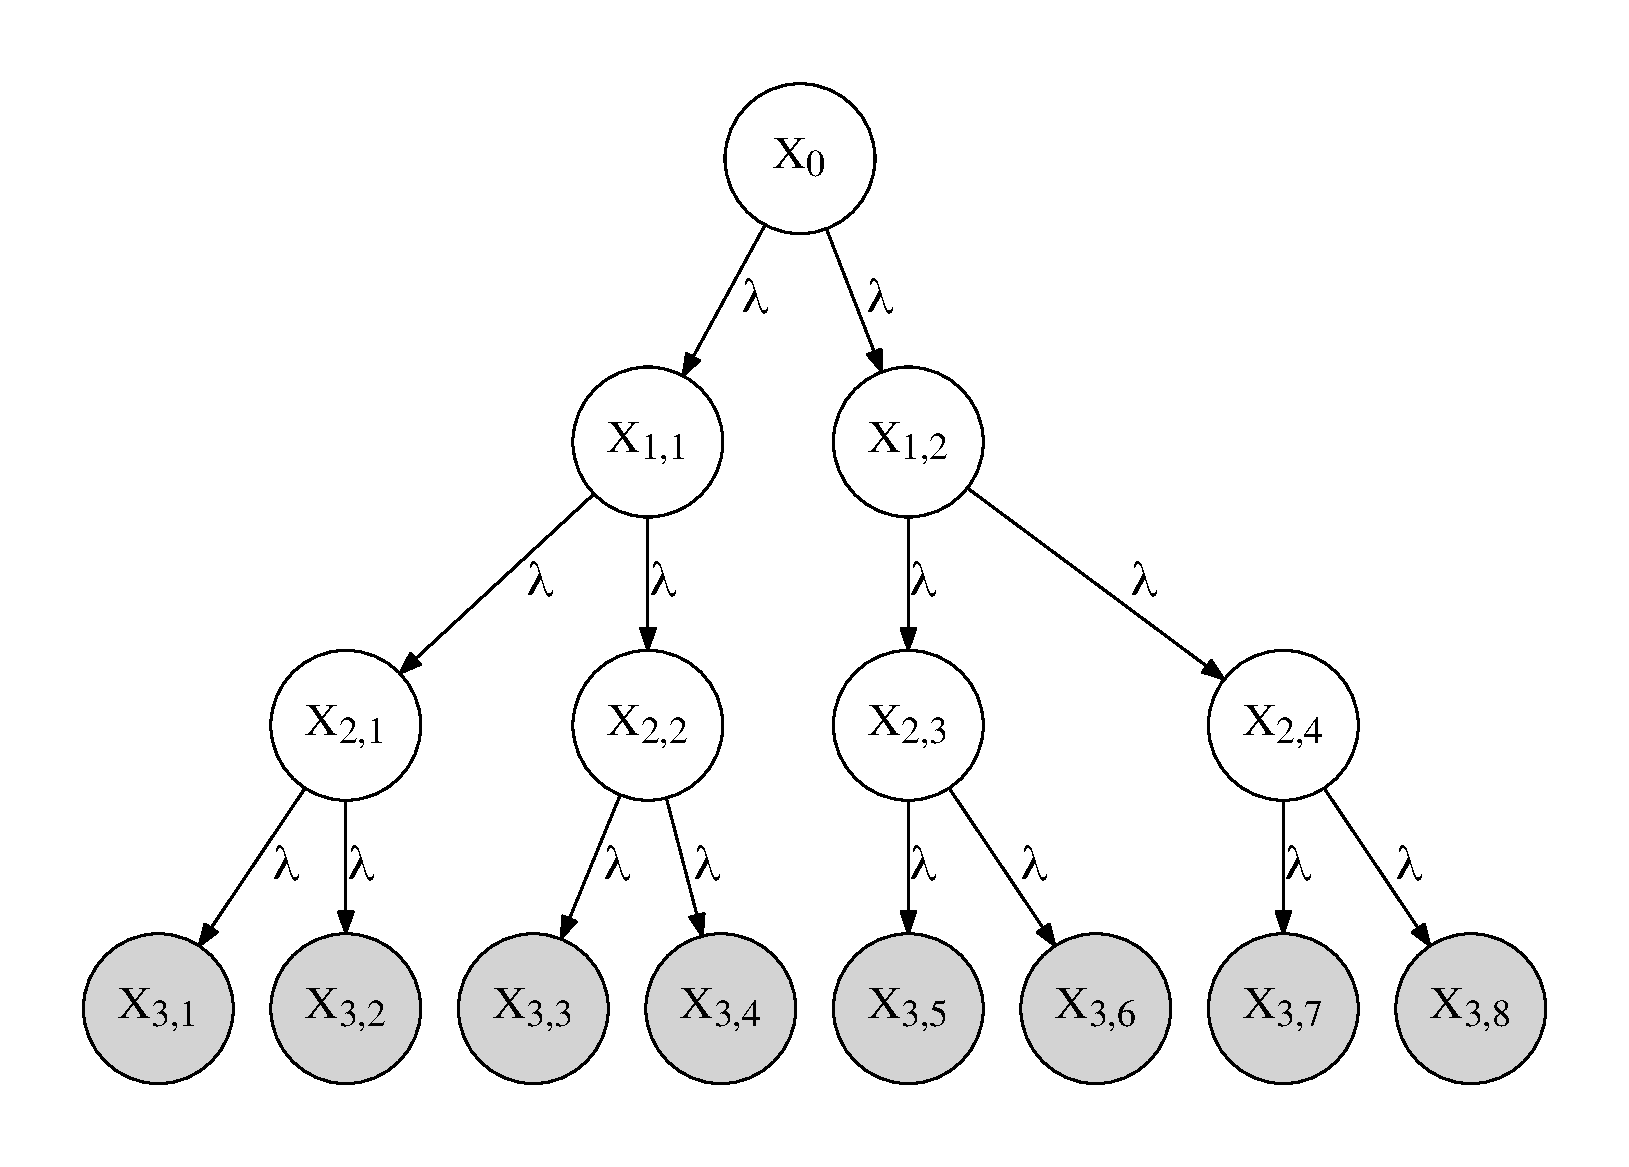
\includegraphics[keepaspectratio=true,width=0.35\textwidth]{tree.pdf}
\caption{ Phylogenetic model for system evolution  with $K=3$ branching events \label{fig:tree}}
\end{figure}

\section{Statement of the problem}
\label{statement of the problem}
The system studied is the following: a balanced phylogenetic tree is given, with $K$ branching events and times $\Delta t_{ij}$ being assigned to each of its branches. A root configuration $\mathbf{x}$ is chosen with gaussian probability 
$$ P_{eq}(\mathbf{x}) = \frac{1}{\sqrt{(2\pi)^N \vert \bm{J}^{-1}\vert}}\exp\left\{ -\frac{1}{2}\mathbf{x}^T\bm{J}\mathbf{x} \right\}. $$ 
It then evolves using Ornstein-Uhlenbeck dynamics which is fully determined by the pairs $\left\lbrace \bm J,\gamma \right\rbrace $. At each division event of the tree, two or more  copies of the system are created and evolve independently along each branch. The final result of the process are the configurations at leaves of the tree. \\
The inference problem is then: with the knowledge of the leaves configurations $\mathbf{y}=\left[ \mathbf{x}_1,\mathbf{x}_2,...,\mathbf{x}_k\right] $ , the tree and  the type of evolution dynamics (O-U evolution), is it possible to reconstruct the potential $\bm J=\bm{C}^{-1}$ acting on the system and the dynamics parameter $\gamma$? 

The Bayesian approach  to this is:
\begin{itemize}
	\item Compute the probability of observing leaves configurations given the potential $\bm{J}$,and mutation rate $1/\gamma$ given by the likelihood: $P(\mathbf{y}\vert\bm{J},\gamma)$.
	\item Compute posterior of the parameters  using Bayes formula: $$P(\bm{J},\gamma\vert \mathbf{y}) = \frac{P(\mathbf{y}\vert\bm{J},\gamma)P(\bm{J},\gamma)}{Z}$$
	\item Maximize  posterior of the model by  maximum likelihood approach: $ \max_{\bm J,\gamma} P(\mathbf{y}\vert\bm{J},\gamma)$  which is exact  when this function is strictly concave and prior distribution is uniform.
\end{itemize}



\section{Methods}
\label{methods}
Since the process is always Gaussian the distribution of the leaves has to be Gaussian itself. Furthermore, we know the covariance between any two elements. Within one leaf, the covariance is the equilibrium covariance $\bm {J}^{-1}$, and among leaves it has to be $\Lambda^{\Delta t_{ij}}{\bm J^{-1}}  $
%\[ {\bm g}_{ij}(\Delta t_{ij},\bm{J}) = \bm \Lambda^{\Delta t_{ij}}{\bm J^{-1}}   \]
with $\bm \Lambda = \exp(-\bm J/\gamma)$ and $\Delta t_{ij}$ is the  path time   between nodes $i$ and $j$ along the branches of the tree.



The distribution of the leaves is given by 
\begin{eqnarray}
\nonumber
\lefteqn{P(\mathbf{y}=\left[ \mathbf{x}_1,\ldots,\mathbf{x}_R\right] ) = \frac 1 {\sqrt{ 2 \pi^{N R} \det \mathbb{G}}  }}\\%\nonumber
&&\times \exp\left(-\frac 1 2 [\mathbf{x}_1,\ldots,\mathbf{x}_R] \mathbb{G}^{-1}[\mathbf{x}_1,\ldots,\mathbf{x}_R]^t \right)
\label{eqn:leaves_dist}
\end{eqnarray}
where $\mathbb{G}$ is a block matrix whose structure is induced by the  phylogenetic tree  and   its elements are given by: 


\begin{equation}
\bm G_{i,j} =
\begin{cases}
\bm J^{-1} & \text{$i=j$}.\\
\bm \Lambda^{\Delta t_{ij}}{\bm J^{-1}} & \text{otherwise}  
\end{cases}
\end{equation}


The log likelihood is
\begin{equation}\label{eq:log_likelihood}
L(\mathbf{y}|\bm J,\gamma) = \frac 1 2 \log \det  \mathbb{G}^{-1}  -\frac 1 2 \mathbf{y}\mathbb{G}^{-1} \mathbf{y}^t
\end{equation}

Trivial maximization over a full fledge $\mathbb{G}$ would give back the experimental correlation between leaves, but it would lack the structure of $\mathbb{G}$. Maximization over $J_{i,j}$ could be attempted through the chain rule
\[  \frac{\partial L}{\partial J_{i,j}} = \sum_{p,q}\frac{\partial L}{\partial G^{-1}_{p,q}} \frac{\partial G^{-1}_{p,q}}{\partial J_{ij}} \]
Although $\frac{\partial L}{\partial G^{-1}_{p,q}}$ is simple to compute, the part $ \frac{\partial G^{-1}_{p,q}}{\partial J_{ij}}$ is not.

To numerically optimize the log likelihood is necessary   to compute  the determinant of  $\mathbb{G}$   for each change in the potential matrix $\bm{J}$.  It is a huge problem for systems of realistic sizes with complexity $O(N^3*R^3)$ where $R$ is the number of leafs in the tree and $N$ the size of configuration vector  $\mathbf{x}_i$. However we could simplify it  using the symmetric properties of  this matrix, as we will show below.
\subsection{Simpler case: Binary and homogeneous tree.}
Let assume that the tree is binary and completely homogeneous, all branches have the same length $\Delta t$. For instance the sequences covariance matrix for a binary tree with $K=2$ branching events and four leaves is
\begin{equation} 
\mathbb{G} =  \left(
\begin{array}{cccc}
{ \bm J^{-1}} & {\bm J^{-1}} \Lambda ^{2\Delta t} & {\bm J^{-1}} \Lambda ^{4\Delta t} & {\bm J^{-1}} \Lambda ^{4\Delta t} \\
{\bm J^{-1}} \Lambda ^{2\Delta t} & {\bm J^{-1}} & {\bm J^{-1}} \Lambda ^{4\Delta t} & {\bm J^{-1}} \Lambda ^{4\Delta t} \\
{\bm J^{-1}} \Lambda ^{4\Delta t} & {\bm J^{-1}} \Lambda ^{4\Delta t} & {\bm J^{-1}} & {\bm J^{-1}} \Lambda ^{2\Delta t} \\
{\bm J^{-1}} \Lambda ^{4\Delta t} & {\bm J^{-1}} \Lambda ^{4\Delta t} & {\bm J^{-1}} \Lambda ^{2\Delta t} & {\bm J^{-1}} \\
\end{array}\label{eq:CL}
\right)
\end{equation}


For hypergeometric matrices as \ref{eq:CL} there is $K+1$ different eigenvalues  given by: 

\begin{equation}
\label{eq:lambda_hyper}
\lambda_k =
\begin{cases}
J^{-1}(1+\sum_{l=1}^{k-1} 2^{l-1}\Lambda^{2l\Delta t}-2^{k-1}\Lambda^{2k\Delta t} )\;\;\; k\in[1,K] \\
J^{-1}(1+\sum_{l=1}^{K} 2^{l-1}\Lambda^{2l\Delta t}) \;\;\;\;\;\;\;k=K+1
\end{cases}
\end{equation}

where $\lambda_{K+1}\ge\lambda_{K}\cdots\ge\lambda_{1}$. For $k<K+1$ degenerancy of eigenvalues $\lambda_k$ is given by : $d_k=2^{K-k}$.  

The associated eigenvectors are independent of potential $\bm J$ and reflects the events in the phylogenetic tree  where each eigenvector  $k$ captures the duplication events in the $(K+1 -k) 	st$ generation. Summarizing :

\begin{equation} 
\nonumber
	\bm u_k =
	\begin{cases}
	{(\underbrace{\overbrace{1,\ldots,1}^{2^{k-1}},\overbrace{-1,\ldots,-1}^{2^{k-1}}}_Q,0,\ldots,0)\ \bigcup \Gamma(u_k) } \;\;\; k\in[1,K] \\
	(1,1,1,\ldots,1,1,1)\;\;\;\;\;\;\;k=K+1
	\label{eq:eigenvec_simpler_case}
\end{cases}	
\end{equation}

where $\Gamma(u_k)$ represent $d_k$ combinations resulting of shift the block of length $Q$ without overlapping, generating all eigenvectors with the same corresponding eigenvalue $\lambda_k$.  The eigenvectors are orthogonal to eachother, and can be  normalized and arranged horizontally into a matrix $U$. With this in mind  the log-likelihood can be written as             
           
\begin{eqnarray}
\nonumber
\lefteqn{L=\frac 1 2 \log\det \mathbb{G} ^{-1}-\frac 1 2 y \mathbb{G} ^{-1}y^t}\\
&&=\frac 1 2 \log\prod_{k}\lambda_k^{-1}  -\frac 1 2 \mathbf{y}  \bm U' \mbox{Diag}\left({\frac 1 \lambda_k}\right) \bm U \mathbf{y}^t \\\nonumber
&&=-\frac 1 2\sum_{k}\log\lambda_k-\sum_k \frac{\langle \mathbf{u}_k | \mathbf{y}\rangle^2}{\lambda_k} 
\end{eqnarray}

\subsection{Likelihood maximization for leaves as  one-dimensional  vectors: N=1}

For one dimension ($N=1$) the log-likelihood can be maximized over the only two parameter  $p_{i=1,2}=\gamma , J = \sigma^{-2}$, being $\sigma$ standard deviation , following the 
gradient
\begin{equation}
\nabla L=\sum_i\frac{\partial L}{\partial p_i}\hat{p_i} 
\end{equation}
with 
\begin{eqnarray}
\nonumber
\label{eq:gradient1D}
\lefteqn{\frac{\partial L}{\partial p_i} = -\sum_{k}^R \frac 1 {\lambda_k} \frac{\partial \lambda_k}{\partial p_i}  +\sum_{k}^R \frac{\langle \mathbf{u}_k | \mathbf{y}\rangle^2}{\lambda_k^2} \frac{\partial \lambda_k}{\partial p_i}} \\ &&= \sum_{k}^R  \left(\frac{\langle \mathbf{u}_k | \mathbf{y}\rangle^2}{\lambda_k} -1 \right) \frac 1 {\lambda_k} \frac{\partial \lambda_k}{\partial p_i}	 
\end{eqnarray}


Using  equation \ref{eq:gradient1D} we implement a gradient ascent method to maximize the log-likelihood of data generated by algorithm \ref{alg_1} with $\gamma_0=1.0$, $\Delta t=0.5 t_c$ and $\sigma_{eq} \sim N(0,1)$ . In the figure below  we show the convexity of the log-likelihood function and the ability of our algorithm to find the value of $ \sigma^2$ which maximizes it ($\sigma^2_{max}$),  being a better approximation for the true  standard deviation ($\sigma^2_{eq}$) than the empirical one ($\sigma^2_{emp}$) .

\begin{figure}[!htb]
	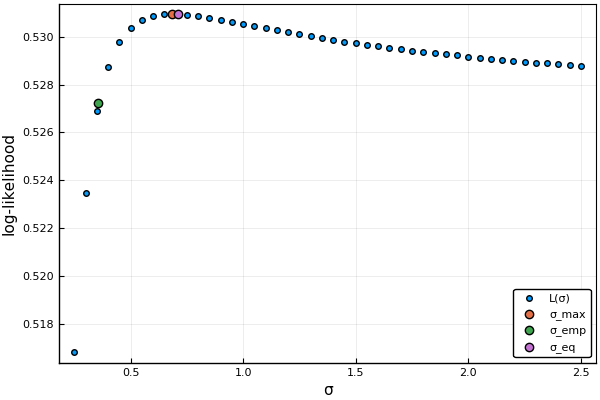
\includegraphics[keepaspectratio=true,width=0.40\textwidth]{log-likelihood_vs_sigma_1D.png}
\caption{ Log-likelihood function for data sampled trough a tree with $R=2^{13} $ and $dt=0.5tc$.}
\end{figure}


\subsection{Generalized inference method: N-dimensional case}
For the most general case the coupling matrix $\bm J$ is a $N\times N$  matrix and as consequence $\mathbb{G}$ a $RN\times RN$ matrix where $N$ is the sequence length and $R$ the leafs number. 
The eigensystem of $\bm J$ allows to write:


$$\bm  J \ket{\textbf{s}_i} =\rho_i\ket{\textbf{s}_i }$$
and
$$\bm J=\sum_{i}\rho_i \ket{\textbf{s}_i}  \bra{\textbf{s}_i}  $$

been $\ket{\textbf{s}_i}$ and $\rho_i$ eigenvectors and eigenvalues of $\bm J$. As each entry $m,n$ of $\mathbb{G}$ is a function of $\bm J$ we have:

$$\mathbb{G}=\bm G_{m n}(\bm J)$$

with $m,n \in (1:R)$ and projecting on $\ket{\textbf{s}_i}$   $$\bm G_{m n}(\bm J)\ket{\textbf{s}_i} =\bm G_{m n}(\rho_i)\ket{\textbf{s}_i} $$  note now that to replace $\bm J$ matriz by it's eigenvalues $\rho_i$   produce $\bm G_{m n}(\rho_i)$ , a hypergeometric matrix  with $\dim(\bm G_{m n}(\rho_i))=R\times R $ and eigensystem ($\lambda_k(\rho_i)$,$\textbf{u}^k(\rho_i)$).  

For a homogeneous and binary phylogenetic tree such as the one presented in figure \ref{fig:tree}, $\lambda_k (\rho_i)$, $\textbf{u}^k(\rho_i) $ are given by the expressions provided by \ref{eq:lambda_hyper} and \ref{eq:eigenvec_simpler_case}, however in general cases $ \lambda_k (\rho_i) $, $\textbf{u}^k(\rho_i)$ must be calculated for every $ i \in (1: N) $

Lets consider the vector built as the Kronecker product  $$\ket{\textbf{u}^{ki}} \otimes\ket{\textbf{s}_i} =(u^{ki}_1 \ket{\textbf{s}_i} \dotsc u^{ki}_R \ket{\textbf{s}_i} )^T=u^{ki}_{\alpha}s^{i}_{\beta}$$
this vectors and the eigenvalues $\lambda_{k}(\rho_i)=\lambda_{k,i}$ conform the eigensystem of the full matrix  $\mathbb{G}$ as is shown below:

\begin{eqnarray*}\mathbb{G}\ket{\textbf{u}^{ki}} \otimes\ket{\textbf{s}_i} &=&\sum_{n}\bm G_{mn}(\bm J)(\ket{\textbf{u}^{ki}} \otimes\ket{\textbf{s}_i})_n\\ &=&\sum_{n}\bm G_{mn}(\bm J)\ket{\textbf{u}^{ki}}_n\otimes\ket{\textbf{s}_i}\\&=&\sum_{n}\bm G_{mn}(\bm J)\ket{\textbf{s}_i}\otimes \ket{\textbf{u}^{ki}}_n\\&=&\sum_{n}\bm G_{mn}(\rho_i)\ket{ \textbf{s}_i} \otimes \ket{\textbf{u}^{ki}}_n\\&=&\sum_{n}\bm G_{mn}(\rho_i)\ket{\textbf{u}^{ki}}_n\otimes\ket{\textbf{s}_i}\\&=&\lambda_k(\rho_i) \ket{\textbf{u}^{ki}}\otimes\ket{\textbf{s}_i}=\lambda_{k,i} u^{ki}_{\alpha}s^{i}_{\beta} 
\end{eqnarray*}


Therefore $$\mathbb{G}\ket{\textbf{u}^{ki}} \otimes\ket{\textbf{s}_i}=\lambda_k(\rho_i) \ket{\textbf{u}^{ki}} \otimes\ket{\textbf{s}_i} $$ 

Then the log likelihood for the general case could be written as:
\begin{equation}
L= -\frac 1 2\sum_{k,i}\log\lambda_{k,i}-\frac 1 2 \sum_{k,i} \frac{\left( \sum_{\alpha,\beta} u^{ki}_{\alpha} s^{i}_{\beta} y_{\alpha\beta} \right) ^2}{\lambda_{k,i}}
\label{eq: log_lik ND}
\end{equation}
where $k,\alpha \in (1:R)$ and $i,\beta \in (1:N)$ then re-arranging the second term we get,


\begin{equation}
L(\mathbf{y}|\rho_i,\mathbf{s}_i,\gamma)= -\frac 1 2\sum_{k,i}\log\lambda_{k,i}-\frac{1}{2}  \sum_{i} \mathbf{s}_i^{T} \mathbf{A}^{i} \mathbf{s}_i
\label{eq: log_lik ND_new_not}
\end{equation}

where 

\begin{equation}
A^{i}_{\beta\delta}=\sum_{k,\alpha,\gamma} \frac{u^{ki}_{\alpha}  u^{ki}_{\gamma}y_{\alpha\beta} y_{\gamma\delta}}{\lambda_{ki}}
\end{equation}

\subsubsection{Regularization}
An $l2$-regularization term, with strength $r_J=10^{-2}$ , is added to expression \ref{eq: log_lik ND_new_not} in order to enforce strict concavity of the log-likelihood function and to remove infinite values of couplings motivated by  overfitting. This term correspond to gaussian prior information describing sparsity of the coupling matrix and leads to the objective function:

\begin{equation}
L(\mathbf{y}|\rho_i,\mathbf{s}_i,\gamma)= -\frac 1 2\sum_{k,i}\log\lambda_{k,i}-\frac{1}{2}  \sum_{i} \mathbf{s}_i^{T} \mathbf{A}^{i} \mathbf{s}_i- r_J*\sum_{i} \rho^2_i
\label{eq: log_lik_ND_regul}
\end{equation}




\subsection{Optimization scheme}


Equation \ref{eq: log_lik_ND_regul}  can be maximized by exploring the space of the coupling matrices by varying its $ N $ eigenvectors $\mathbf{s}_i$  and $ N $ eigenvalues $\rho_i$ in the positive direction of the log likelihood gradient .

As $ \mathbf{s}_i$ is a basis set in an n-dimensional linear space,  our optimization problem is subject to the orthogonality constraint on the set $ \mathbf{s}_i,i=1,2,...,N$. This implies that the transformation of a base formed by the vectors $\mathbf{s}_i$ is established by an orthogonal matrix. 

An arbitrary orthogonal matrix $\bm S$ can be parameterized  representing its elements in terms of $N(N-1)/2$ independent variables $ \left\lbrace \bm \phi\right\rbrace $ and then each base vector is parameterized according to the $ith$ column of the  matrix. Optimization of log-likelihood,  $L(\boldmath{\bm \phi})\equiv L(\bm S(\boldmath{\bm \phi})) $, on these variables will impose on our problem the  orthogonality constraint without  to introduce Lagrange multipliers in our variational problem. Gradients of the scalar function on this variables  must be computed using the chain-rule transformation:

\begin{equation}
\frac{\partial L}{\partial \phi_\mu}=\sum_{p,q} \frac{\partial L}{\partial S_{p,q}}\frac{\partial S_{p,q}}{\partial \phi_\mu}
\end{equation}

There are several methods to perform this procedure \cite{Shepard_param_OM}, we implement here a parameterization algorithm of an orthogonal matrix in terms of generalized Eulerian angles \cite{Raffenetti1970GEA}, which establishes a recursive procedure that allows the computation of matrix elements as a function of $N(N-1)/2$  independent angular variables $\theta_ {pq}, p =1,2, ..., N; q =1,2, ..., N; p <q $, and also the orthogonal matrix derivative with respect to these angular variables. This allow to compute the gradient as:


\begin{equation}
\nabla L=\sum_i\frac{\partial L}{\partial \rho_i}\hat{\rho_i} +\sum_{p,q}\frac{\partial L}{\partial \theta_{pq}}  \hat{\theta}_{pq} +\frac{\partial L}{\partial \gamma}\hat{\gamma} 
\end{equation}

where 
\begin{equation}
\frac{\partial L}{\partial \rho_i} = -\frac{1}{2}\left\lbrace  \sum_k \frac{1}{\lambda_{ki}}\frac{\partial \lambda_{ki}}{\partial\rho_i} +\mathbf{s}_i^{T} \frac{\partial \mathbf{A}^{i} }{\partial\rho_i}\mathbf{s}_i \right\rbrace -2 r_{J} \rho_i
\end{equation}

\begin{equation}
\frac{\partial L}{\partial \gamma} = -\frac{1}{2}\left\lbrace  \sum_{k,i} \frac{1}{\lambda_{ki}}\frac{\partial \lambda_{ki}}{\partial\gamma} +\mathbf{s}_i^{T} \frac{\partial \mathbf{A}^{i} }{\partial\gamma}\mathbf{s}_i \right\rbrace 
\end{equation}


and

\begin{equation}
\frac{\partial L}{\partial \theta_{p,q} }=-\sum_{i} \frac{\partial \mathbf{s}_i^{T} }{\partial \theta_{p,q} } \mathbf{A}^{i}  \mathbf{s}_i
\end{equation}


For  gradient evaluation,derivatives of the eigenvalues $\lambda_ {k, i} $ and eigenvectors $u^{k, i}_{\alpha} $ of the matrix $\bm G(\rho_i) $ respect $\rho_i$ parameter must be computed:

\begin{eqnarray}
\nonumber
\lefteqn{\frac{\partial \mathbf{A}^{i} }{\partial\rho_i}=2 \sum_{k} \frac{1}{\lambda_{k,i}}\sum_{\alpha} (u_{\alpha}^{k,i})' y_{\alpha\beta}\sum_{\gamma} u^{k,i}_{\gamma} y_{\gamma\delta}}\\&&-\frac{1}{\lambda_{k,i}^2} \lambda'_{k,i}\sum_{\alpha}u^{k,i}_{\alpha}y_{\alpha\beta}\sum_{\gamma} u^{k,i}_{\gamma} y_{\gamma\delta}
\end{eqnarray}
where 


\begin{equation}\lambda'_{k,i}=\frac{\partial \lambda_k(\rho_i) }{\partial\rho_i}\end{equation}

\begin{equation}(u_{\alpha}^{k,i}) ' =\frac{\partial u^{k}_{\alpha}(\rho_i) }{\partial\rho_i}\end{equation}


If the eigenvalues $\lambda_k(\rho_i)$ and eigenvectors $\bm{u}^{k}(\rho_i)$ of  $\bm G(\rho_i)$ are  already available and all eigenvalues are distinct (as in the case of a non-homogenous phylogenetic tree) a simple analytical expression can be derived for the calculation of its corresponding derivatives with respect to the $\rho_i$ parameter \cite{matrix_cook_book} :

\begin{equation}
\frac{\partial \lambda_k(\rho_i) }{\partial\rho_i}=\bm{u}^{k}(\rho_i) ^T\frac{\partial \bm G(\rho_i) }{\partial\rho_i} \bm {u}^{k}(\rho_i) 
\end{equation}
\begin{eqnarray}
\nonumber
\frac{\partial u^{k}_{\alpha}(\rho_i)}{\partial\rho_i}=\sum_{p\neq k}\frac{\left( u^{p}_{\alpha}(\rho_i)^T\frac{\partial \bm G(\rho_i) }{\partial\rho_i} u^{k}_{\alpha}(\rho_i)\right) }{\lambda_{k}(\rho_i)-\lambda_{p}(\rho_i)} u^{p}_{\alpha}(\rho_i)
\end{eqnarray}

Using previous expressions it is possible to maximize the log-likelihood \ref{eq: log_lik_ND_regul}  over parameters: $\gamma$, $\rho_i, i = 1,2, .. N $ and $\theta_ {pq}, p = 1,2, ..., N; q = 1,2,..., N; p <q $. This nonlinear optimization problem was addressed by implementing a quasi-Newton Method algorithms \cite{NLopt}.
\subsection{Initializing parameters}
From empirical covariance matrix $c^*=\frac{1}{N}\sum_{n=1}^{N}\mathbf{x}_n \mathbf{x}_n^T$ we could extract information  to  initialize the parameters in the optimization process. 

The eigenvalues of empirical couplings $j^*=1/c^*$  will define $\rho^0_i$ ands its eigenvectors  an orthogonal matrix $\bm S^0$ which satisfy the equations systems:
\begin{equation}
S_{ij}(\theta^0)=S^0_{ij}
\label{recurrent_eq}
\end{equation}
to find the orthogonal parameters which reproduce the initial orthogonal matrix, equation \ref{recurrent_eq} must be inverted or equivalently the solution set $\bm \theta^0$ could be numerically obtained minimizing the function:

\begin{equation}
f(\bm \theta^0)=\sum_{i,j}\left[ S^0_{ij}-S_{ij}(\bm \theta^0)\right] ^2
\label{obtain_theta0}
\end{equation}

\subsubsection{Empirical parameter $\gamma_0$}
The probability distribution for two leaves $\mathbf{x}_1$ and  $\mathbf{x}_2$  separated by time $t_{12}$ , $P(\mathbf{x}_1,\mathbf{x}_2|t_{12})$ is given by the equation (12) for $R=2$. With this distribution we can calculate analytically the average of the scalar product $\mathbf{x}_1\cdot\mathbf{ x}_2$:

\begin{eqnarray}
\nonumber
\lefteqn{\left\langle \mathbf{x}_1\cdot\mathbf{ x}_2\right\rangle = \int \mathbf{dx}_1 \mathbf{dx}_2 \sum_{i} x_1(i) x_2(i)  P(\mathbf{ x}_1,\mathbf{ x}_2|t_{12})}\\\nonumber&&=\sum_{i} \left\langle  x_1(i) x_2(i)\right\rangle_{t_{12}}
=\sum_{i} \left( \bm \Lambda^{t_{12}} \bm J^{-1}\right)_{ii}=\Tr \left(\bm \Lambda^{t_{12}} \bm J^{-1} \right)  
\end{eqnarray}

If the eigensystem of $\bm J$ is known : $\left\lbrace\rho_i, \mathbf{s}_i\right\rbrace $, we get:

\begin{equation}
\left\langle \mathbf{ x}_1\cdot\mathbf{ x}_2\right\rangle =\Tr \left(\bm \Lambda^{t_{12} } \bm J^{-1}\right) =\sum_{i} \frac{ e^{-\frac{\rho_i t_{12}}{\gamma}}}{\rho_i}
\end{equation}


then as we know from the data the empirical values of the pairs $\left\lbrace t,\mathbf{ x}_1\cdot\mathbf{x}_2 \right\rbrace $ we could fit the parameter $\gamma$ minimizing the  function:

\begin{equation}
F(\gamma)=\sum_{a,b}\left[\mathbf{ x}_b\mathbf{ x}_b -\sum_{i} \frac{e^{-\frac{\rho_i t_{a,b}}{\gamma}}}{\rho_i}\right] ^2
\label{gamma_inverse_eq}
\end{equation}

using $\rho_i^0$ in minimization of \ref{gamma_inverse_eq} we obtain the empirical value $\gamma_0$.

An algorithm based on gradient descent method is used  to minimize functions \ref{obtain_theta0} and \ref{gamma_inverse_eq}.
\section{ Results}
\label{Results}
In order to test the methodology developed , we generate  data according to algorithm \ref{alg_1} using a non-homogeneous tree with branch length randomly selected,  root configuration was drawn from a Gaussian distribution $P^0(\mathbf{ x})\sim N(0,\bm J^{-1})$. The couplings matrix was selected as a positive semidefinite matrix drawn from a normal distribution with $\mu_J=0.8$ and $\sigma_{J}=0.2$. To make the matrix sparse we dilute the couplings with density $0.3$. 

We choose three different values of parameter $\gamma$ in order to simulate  different regimes: with weak  $\gamma_w=0.1\gamma_c$ ,intermediate $\gamma_i=0.3\gamma_c$ and  strong  $\gamma_s=0.5\gamma_c$  phylogenetic signal. For each different  regime, $30$ repetitions  for the sampling-inference process were made obtaining covariance and coupling matrices using our inference procedure and the empirical estimators.

In figures \ref{results_gamma10_n10},  \ref{results_corr_map_J_10_n10}, \ref{results_corr_map_C_10_n10} we compare the two estimation procedure in term of distance and correlation with the original parameters. As can be seen in   our method is able of inferring covariance and  coupling matrices closer to the equilibrium ones for all regimes, and  differences are more clear if there is more phylogeny contamination in  alignments. 

On the other hand if we use the original coupling matrix to create a  contact map between sites, assuming as contact non zero entries, then we could explore the ability of our method to predict topology of the coevolutionary network.  Figure \ref{PPV_n10} show positive predictive values averaged over 30 samples, been the   log-likelihood maximization  a better approach to the contact structure of the original couplings matrix.


 About computations made is useful highlight that as  small dimensions matrices were chosen ( $N=10$) these are not sparse enough, so the prediction of contacts may not be sufficiently enlightening in the comparison. 

\section{Conclusions }
\label{conc}

\textbf{Acknowledgments:} 



\begin{figure*}[!htb]
	\begin{minipage}[b]{0.325\textwidth}
		\begin{center}
			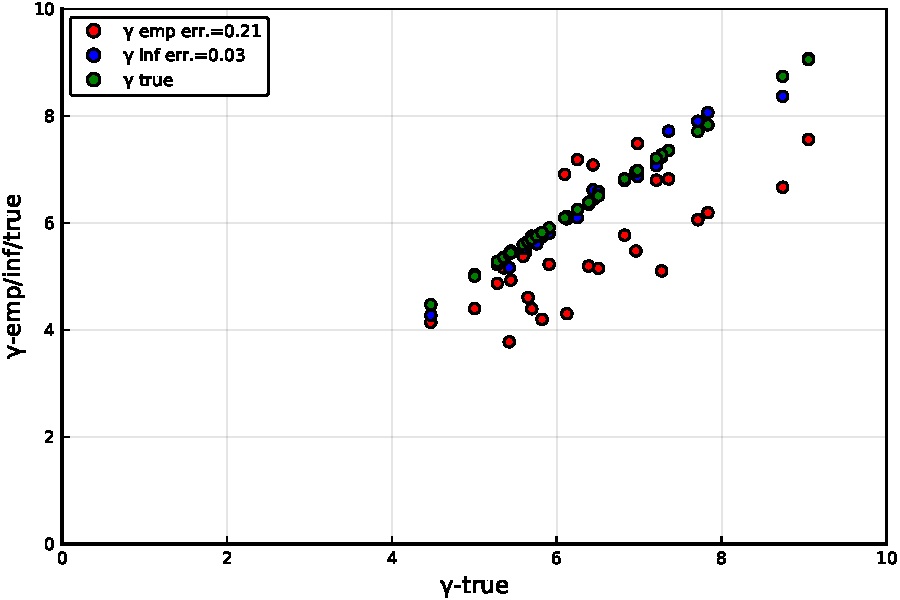
\includegraphics[keepaspectratio=true,width=1\textwidth]{gamma_N10_M1024_optJ_30samp_gamma_c_error_label.pdf}
		\end{center}
	\end{minipage}
	%-------------------------------------
	%-------------------------------------
	\begin{minipage}[b]{0.325\textwidth}
		\begin{center}
			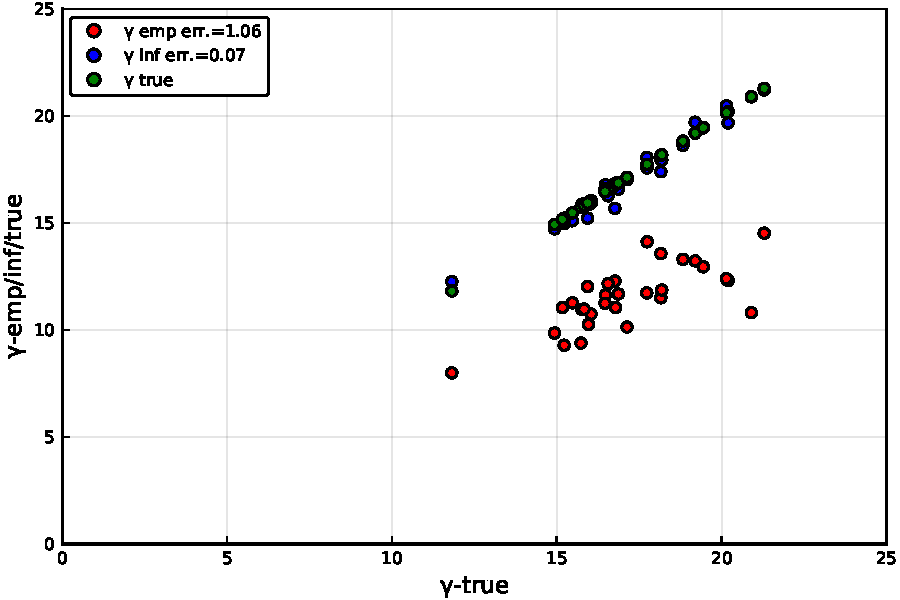
\includegraphics[keepaspectratio=true,width=1\textwidth]{gamma_N10_M1024_optJ_30samp_3gamma_c_error_label.pdf}
		\end{center}
	\end{minipage}
	%-------------------------------------
	%-------------------------------------
	\begin{minipage}[b]{0.325\textwidth}
		\begin{center}
			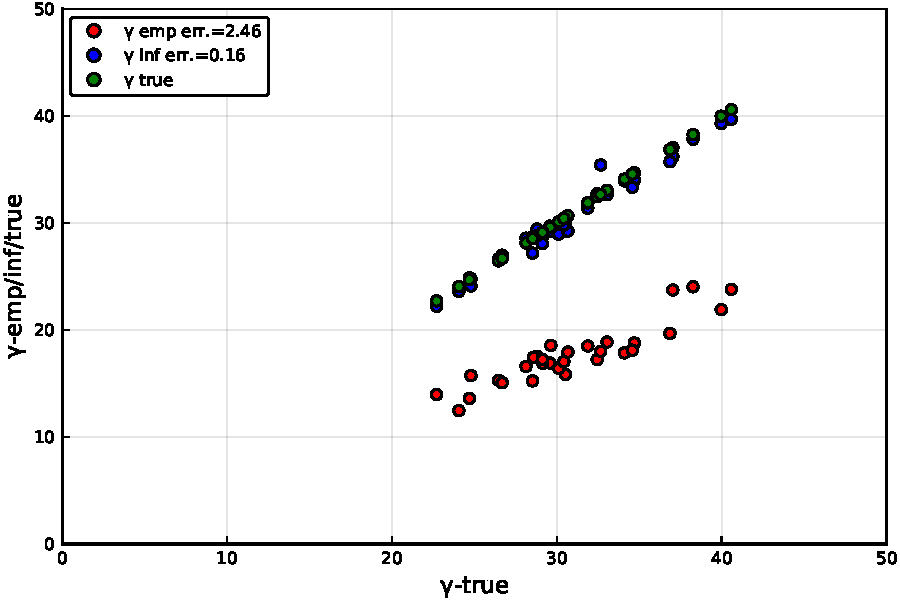
\includegraphics[keepaspectratio=true,width=1\textwidth]{gamma_N10_M1024_optJ_30samp_5gamma_c_error_label.pdf}
		\end{center}
	\end{minipage}
	
	\vspace{-1mm}
	\caption{{ Inference of parameters $\gamma$ for $N=10$ and tree diferent regimes \textbf{left}: $\gamma=\gamma_w$, \textbf{center}: $\gamma=\gamma_i$, \textbf{right} $\gamma=\gamma_s$  }} .
	\label{results_gamma10_n10}
\end{figure*}



\begin{figure*}[!htb]
	\begin{minipage}[b]{0.325\textwidth}
		\begin{center}
			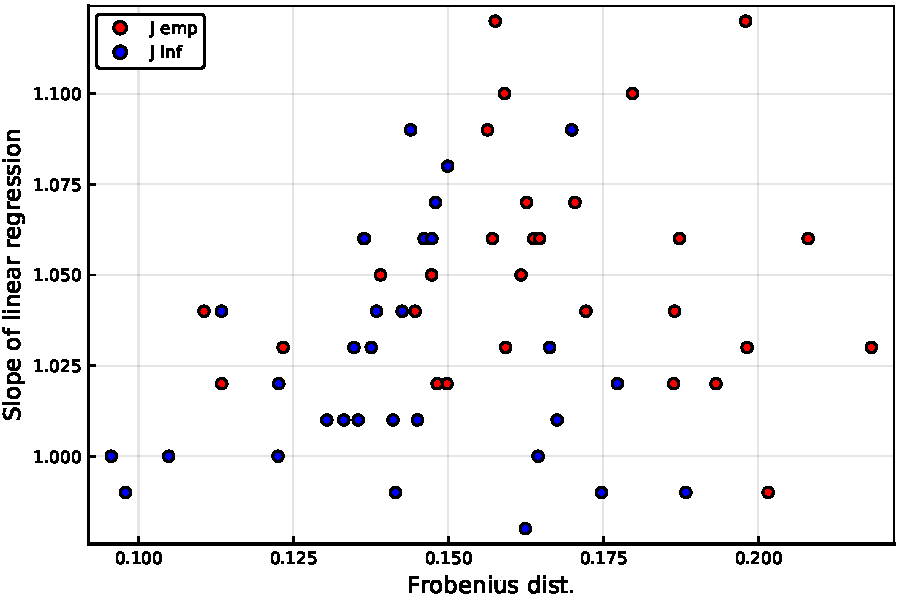
\includegraphics[keepaspectratio=true,width=1\textwidth]{frob_dist_vs_pearson_coup_N10_M1024_optJ_30samp_gamma_c.pdf}
		\end{center}
	\end{minipage}
	%-------------------------------------
	%-------------------------------------
	\begin{minipage}[b]{0.325\textwidth}
		\begin{center}
			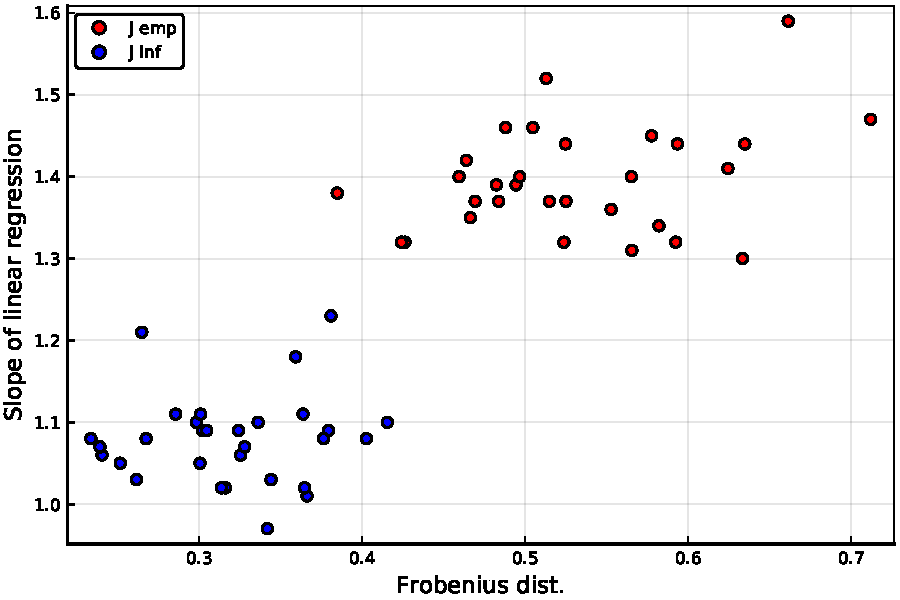
\includegraphics[keepaspectratio=true,width=1\textwidth]{frob_dist_vs_pearson_coup_N10_M1024_optJ_30samp_3gamma_c.pdf}
		\end{center}
	\end{minipage}
	%-------------------------------------
	%-------------------------------------
	\begin{minipage}[b]{0.325\textwidth}
		\begin{center}
			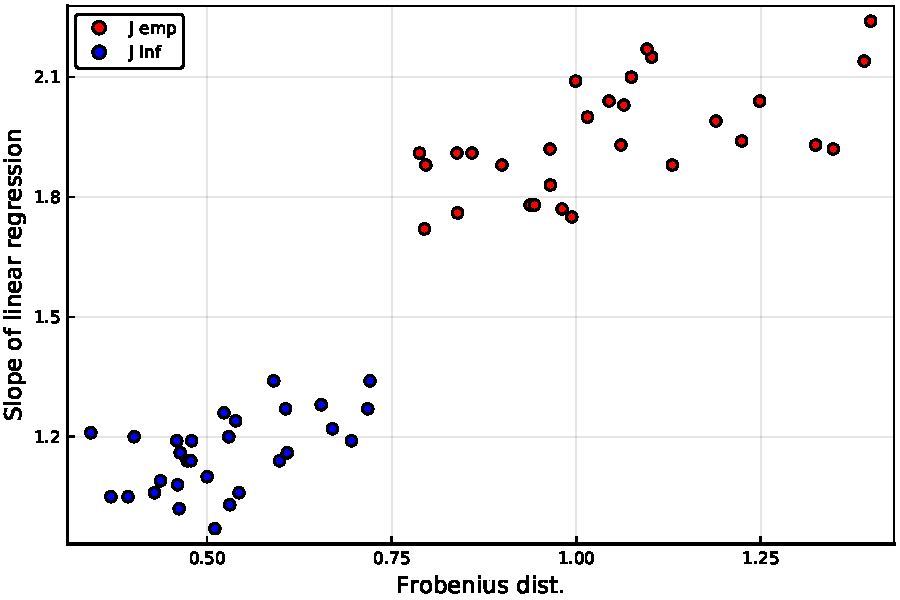
\includegraphics[keepaspectratio=true,width=1\textwidth]{frob_dist_vs_pearson_coup_N10_M1024_optJ_30samp_5gamma_c.pdf}
		\end{center}
	\end{minipage}
	
	\vspace{-1mm}
	\caption{{ Fobenious distance vs slope of linear regression between empirical/infered couplings matrix and true couplings matrix   for $N=10$ and tree diferent regimes \textbf{left}: $\gamma=\gamma_w$, \textbf{center}: $\gamma=\gamma_i$, \textbf{right} $\gamma=\gamma_s$  }} .
	\label{results_corr_map_J_10_n10}
\end{figure*}


\begin{figure*}[!htb]
	\begin{minipage}[b]{0.325\textwidth}
		\begin{center}
			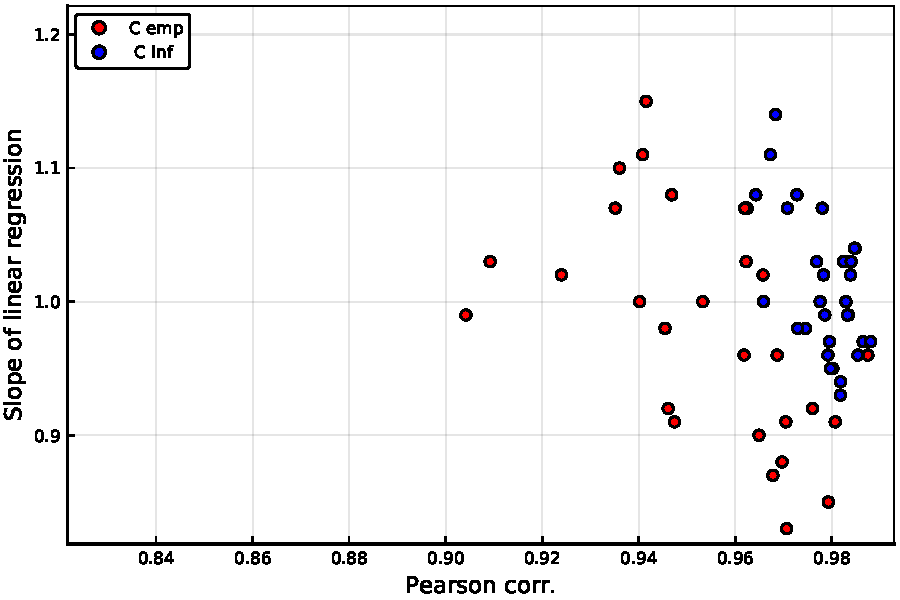
\includegraphics[keepaspectratio=true,width=1\textwidth]{lin_reg_vs_pearson_corr_N10_M1024_optJ_30samp_gamma_c.pdf}
		\end{center}
	\end{minipage}
	%-------------------------------------
	%-------------------------------------
	\begin{minipage}[b]{0.325\textwidth}
		\begin{center}
			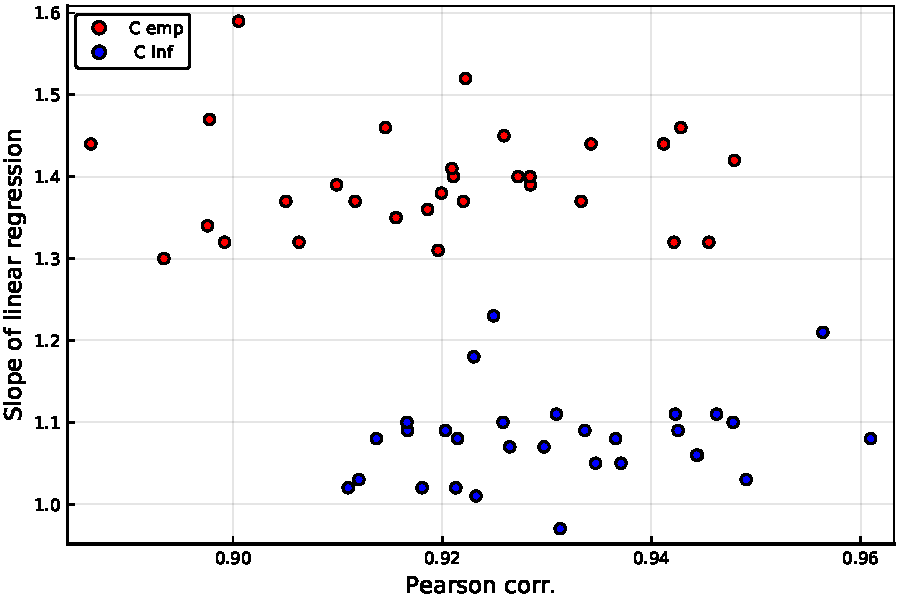
\includegraphics[keepaspectratio=true,width=1\textwidth]{lin_reg_vs_pearson_corr_N10_M1024_optJ_30samp_2gamma_c.pdf}
		\end{center}
	\end{minipage}
	%-------------------------------------
	%-------------------------------------
	\begin{minipage}[b]{0.325\textwidth}
		\begin{center}
			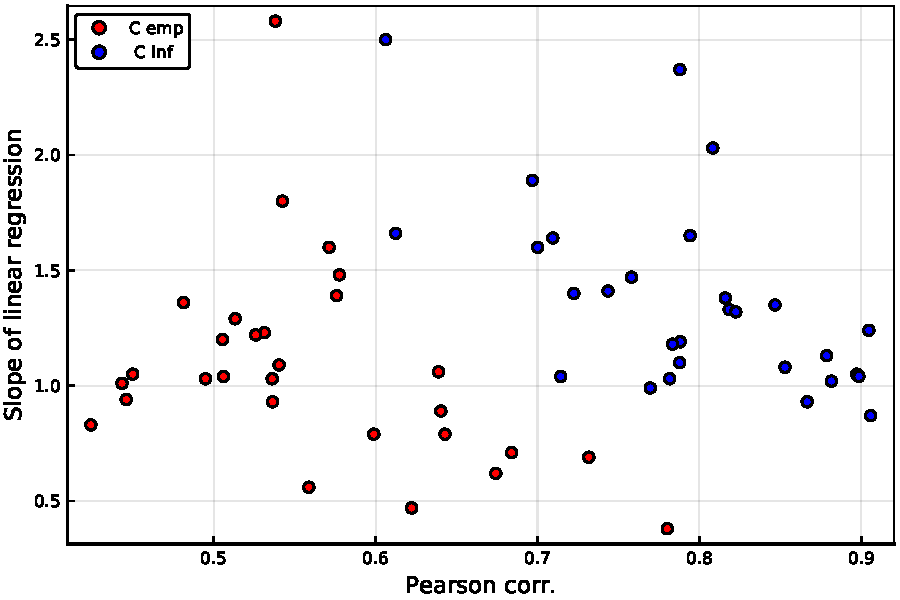
\includegraphics[keepaspectratio=true,width=1\textwidth]{lin_reg_vs_pearson_corr_N10_M1024_optJ_30samp_5gamma_c.pdf}
		\end{center}
	\end{minipage}
	
	\vspace{-1mm}
	\caption{{   Pearson correlation vs slope of linear regression between empirical/infered covariance matrix and true couplings matrix   for $N=10$ and tree diferent regimes \textbf{left}: $\gamma=\gamma_w$, \textbf{center}: $\gamma=\gamma_i$, \textbf{right} $\gamma=\gamma_s$  }} .
	\label{results_corr_map_C_10_n10}
\end{figure*}

\begin{figure*}[!htb]
	\begin{minipage}[b]{0.325\textwidth}
		\begin{center}
			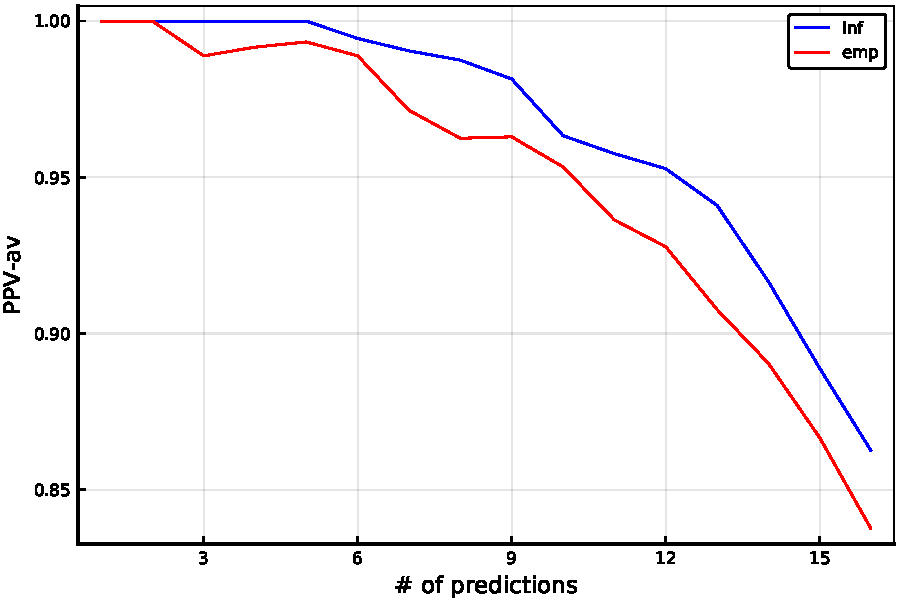
\includegraphics[keepaspectratio=true,width=1\textwidth]{PPV_av30_N10_M1024_optJ_gamma_c_no_diag.pdf}
		\end{center}
	\end{minipage}
	%-------------------------------------
	%-------------------------------------
	\begin{minipage}[b]{0.325\textwidth}
		\begin{center}
			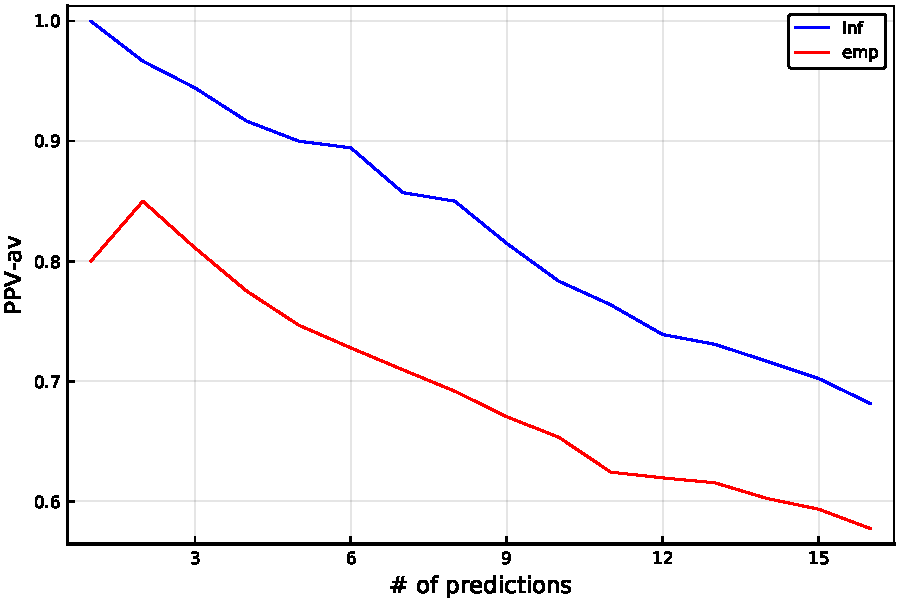
\includegraphics[keepaspectratio=true,width=1\textwidth]{PPV_av30_N10_M1024_optJ_3gamma_c_no_diag.pdf}
		\end{center}
	\end{minipage}
	%-------------------------------------
	%-------------------------------------
	\begin{minipage}[b]{0.325\textwidth}
		\begin{center}
			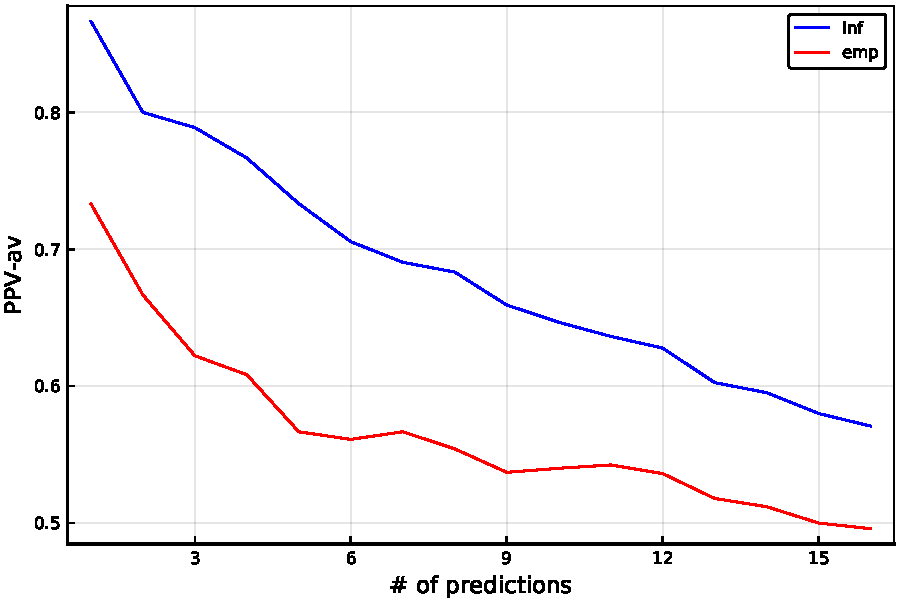
\includegraphics[keepaspectratio=true,width=1\textwidth]{PPV_av30_N10_M1024_optJ_5gamma_c_no_diag.pdf}
		\end{center}
	\end{minipage}
	
	\vspace{-1mm}
	\caption{{  Positive predictive values averaged over 30 samples,  for $N=10$ and tree diferent regimes \textbf{left}: $\gamma=\gamma_w$, \textbf{center}: $\gamma=\gamma_i$, \textbf{right} $\gamma=\gamma_s$  }} .
	\label{PPV_n10}
\end{figure*}




%\begin{figure*}[!htb]
%	\begin{minipage}[b]{0.325\textwidth}
%		\begin{center}
%			\includegraphics[keepaspectratio=true,width=1\textwidth]{Images/new_im/cor_scatter_n6_M1024_gamma10_37samp.png}
%		\end{center}
%	\end{minipage}
%	%-------------------------------------
%	%-------------------------------------
%	\begin{minipage}[b]{0.325\textwidth}
%		\begin{center}
%			\includegraphics[keepaspectratio=true,width=1\textwidth]{Images/new_im/frob_dist_vs_slope_C_n6_gamma10_37samples.png}
%		\end{center}
%	\end{minipage}
%	%-------------------------------------
%	%-------------------------------------
%	\begin{minipage}[b]{0.325\textwidth}
%		\begin{center}
%			\includegraphics[keepaspectratio=true,width=1\textwidth]{Images/new_im/cor_corr_map_n6_M1024_gamma10_37samp.png}
%		\end{center}
%	\end{minipage}
%	\\
%	\vspace{1mm}
%	\begin{minipage}[b]{0.325\textwidth}
%		\begin{center}
%			\includegraphics[keepaspectratio,width=1\textwidth]{Images/new_im/frob_dist_vs_slope_J_n6_gamma10_37samples.png}
%		\end{center}
%	\end{minipage}
%	%-------------------------------------
%	%-------------------------------------
%	\begin{minipage}[b]{0.325\textwidth}
%		\begin{center}
%			\includegraphics[keepaspectratio=true,width=1\textwidth]{Images/new_im/coup_corr_map_n6_M1024_gamma10_37samp.png}
%		\end{center}
%	\end{minipage}
%	%-------------------------------------
%	%-------------------------------------
%	\begin{minipage}[b]{0.325\textwidth}
%		\begin{center}
%			\includegraphics[keepaspectratio=true,width=1\textwidth]{Images/new_im/coup_ppv_n6_M1024_gamma10_37samp.png}
%		\end{center}
%	\end{minipage}
%	\\
%	\vspace{-1mm}
%	\caption{{ covariance and coupling matrices comparison for the regime with weak phylogenetic bias:$N=6$ and $\gamma=10$   }}
%	\label{results_gamma10_n6}
%\end{figure*}
%
%
%
%\begin{figure*}[!htb]
%	\begin{minipage}[b]{0.325\textwidth}
%		\begin{center}
%			\includegraphics[keepaspectratio=true,width=1\textwidth]{Images/new_im/cor_scatter_n6_M1024_gamma100_37samp.png}
%		\end{center}
%	\end{minipage}
%	%-------------------------------------
%	%-------------------------------------
%	\begin{minipage}[b]{0.325\textwidth}
%		\begin{center}
%			\includegraphics[keepaspectratio=true,width=1\textwidth]{Images/new_im/frob_dist_vs_slope_C_n6_gamma100_37samples.png}
%		\end{center}
%	\end{minipage}
%	%-------------------------------------
%	%-------------------------------------
%	\begin{minipage}[b]{0.325\textwidth}
%		\begin{center}
%			\includegraphics[keepaspectratio=true,width=1\textwidth]{Images/new_im/cor_corr_map_n6_M1024_gamma100_37samp.png}
%		\end{center}
%	\end{minipage}
%	\\
%	\vspace{1mm}
%	\begin{minipage}[b]{0.325\textwidth}
%		\begin{center}
%			\includegraphics[keepaspectratio=true,width=1\textwidth]{Images/new_im/frob_dist_vs_slope_J_n6_gamma100_37samples.png}
%		\end{center}
%	\end{minipage}
%	%-------------------------------------
%	%-------------------------------------
%	\begin{minipage}[b]{0.325\textwidth}
%		\begin{center}
%			\includegraphics[keepaspectratio=true,width=1\textwidth]{Images/new_im/coup_scatter_n6_M1024_gamma100_37samp.png}
%		\end{center}
%	\end{minipage}
%	%-------------------------------------
%	%-------------------------------------
%	\begin{minipage}[b]{0.325\textwidth}
%		\begin{center}
%			\includegraphics[keepaspectratio=true,width=1\textwidth]{Images/new_im/coup_ppv_n6_M1024_gamma100_37samp.png}
%		\end{center}
%	\end{minipage}
%	\\
%	\vspace{-1mm}
%	\caption{{ covariance and coupling matrices comparison for the regime with strong phylogenetic bias: $N=6$ and $\gamma=100$   }}
%	\label{results_gamma100_n6}
%\end{figure*}
%
%\begin{figure*}[!htb]
%	\begin{minipage}[b]{0.325\textwidth}
%		\begin{center}
%			\includegraphics[keepaspectratio=true,width=1\textwidth]{Images/new_im/gamma_N10_M1024_optJandC_36sim.pdf}
%		\end{center}
%	\end{minipage}
%	%-------------------------------------
%	%-------------------------------------
%	\begin{minipage}[b]{0.325\textwidth}
%		\begin{center}
%			\includegraphics[keepaspectratio=true,width=1\textwidth]{Images/new_im/frob_dist_vs_pearson_corr_N10_M1024_optJandC_36sim.pdf}
%		\end{center}
%	\end{minipage}
%	%-------------------------------------
%	%-------------------------------------
%	\begin{minipage}[b]{0.325\textwidth}
%		\begin{center}
%			\includegraphics[keepaspectratio=true,width=1\textwidth]{Images/new_im/lin_reg_vs_pearson_corr_N10_M1024_optJandC_36sim.pdf}
%		\end{center}
%	\end{minipage}
%	\\
%	\vspace{1mm}
%	\begin{minipage}[b]{0.325\textwidth}
%		\begin{center}
%			\includegraphics[keepaspectratio=true,width=1\textwidth]{Images/new_im/frob_dist_vs_pearson_coup_N10_M1024_optJandC_36sim.pdf}
%		\end{center}
%	\end{minipage}
%	%-------------------------------------
%	%-------------------------------------
%	\begin{minipage}[b]{0.325\textwidth}
%		\begin{center}
%			\includegraphics[keepaspectratio=true,width=1\textwidth]{Images/new_im/scatter_all_coup_mat_N10_M1024_optJ_andC_36sim.pdf}
%		\end{center}
%	\end{minipage}
%	%-------------------------------------
%	%-------------------------------------
%	\begin{minipage}[b]{0.325\textwidth}
%		\begin{center}
%			\includegraphics[keepaspectratio=true,width=1\textwidth]{Images/new_im/PPV_av_N10_M1024_optJandC_36sim.pdf}
%		\end{center}
%	\end{minipage}
%	\\
%	\vspace{-1mm}
%	\caption{{ covariance and coupling matrices comparison for :$N=10$ and $\gamma=10$   }}
%	\label{results_gamma10_n10}
%\end{figure*}


\newpage

\bibliography{bib_phylo}

\bibliographystyle{unsrt}




\end{document}

